\documentclass[aspectratio=169,12pt,notheorems]{beamer}

\usepackage[utf8x]{inputenc}
\usepackage[russian]{babel}
\usepackage{amsmath,amssymb,amsthm,mathtools}
\usepackage{graphicx,caption,subcaption}
\usepackage{hyperref,natbib}
\usepackage{tikz,xcolor}
\usepackage{algorithm,algpseudocode}

\theoremstyle{plain}
\newtheorem{theorem}{Theorem}
\newtheorem{lemma}[theorem]{Lemma}

\theoremstyle{definition}
\newtheorem{definition}{Definition}
\newtheorem{problem}{Problem}

\usetheme[height=0.95cm]{Rochester}
\usecolortheme{dolphin}

\definecolor{hard}{RGB}{24,15,148}

\setbeamercolor{headline}{bg=hard,fg=white}
\setbeamercolor*{frametitle}{parent=headline}

\setbeamercolor{structure}{fg=hard}
\setbeamercolor{subsection in head/foot}{bg=white,fg=hard}
\setbeamercolor{section in head/foot}{bg=hard,fg=white}
\setbeamercolor{block title}{bg=hard,fg=white}

\setbeamertemplate{navigation symbols}{}

\def\scolon{\rlap{,}\raisebox{0.8ex}{,} }
\def\mitem{\medskip\item}
\def\ps{\\ [0.65cm]} \linespread{1.16}

\def\ll{\left(} \def\rr{\right)}
\def\lag{\left\langle} \def\rag{\right\rangle}

\DeclareMathOperator{\ans}{\text{\scshape ans}}

\title[Incremental Voronoi Diagrams]
	{\bfseries Incremental (Combinatorial)
	     Voronoi Diagrams}

\author[\ ]
	{Boris Zolotov, Mag. 1 \\ \vspace{0.3cm}
		{\small Modern Methods in Computer Science}}

\institute[\ ]{\ }

\date{February 11, 2020}

%%%%%%%%%%%%%%
%%%%%%%%%%%%%%

\begin{document}
\def\mC{\mathcal C} \def\mF{\mathcal F}
\def\mE{\mathcal E} \def\mG{\mathcal G}

\frame{\titlepage}

\begin{frame} \frametitle{Voronoi Diagrams} \label{pg:definition}
\vspace{-0.24cm}

\begin{definition}
	\emph{Voronoi diagram} of set $S \subset \mathbb R^2$ of $n$ points is the subdivision
	of the plane into $n$ \emph{cells}, one for each site in $S$, with the property that
	a point $q$ lies in the cell corresponding to a site $s_i$ if and only if \vspace{-0.5cm}

	$$\mathrm{dist} (q, s_i) < \mathrm{dist} (q, s_j)$$ \vspace{-0.8cm}

	for each $s_j \in S$ with $j \ne i$.
\end{definition}

\begin{figure}[h] \centering
	\begin{subfigure}[t]{0.32\textwidth} \centering
		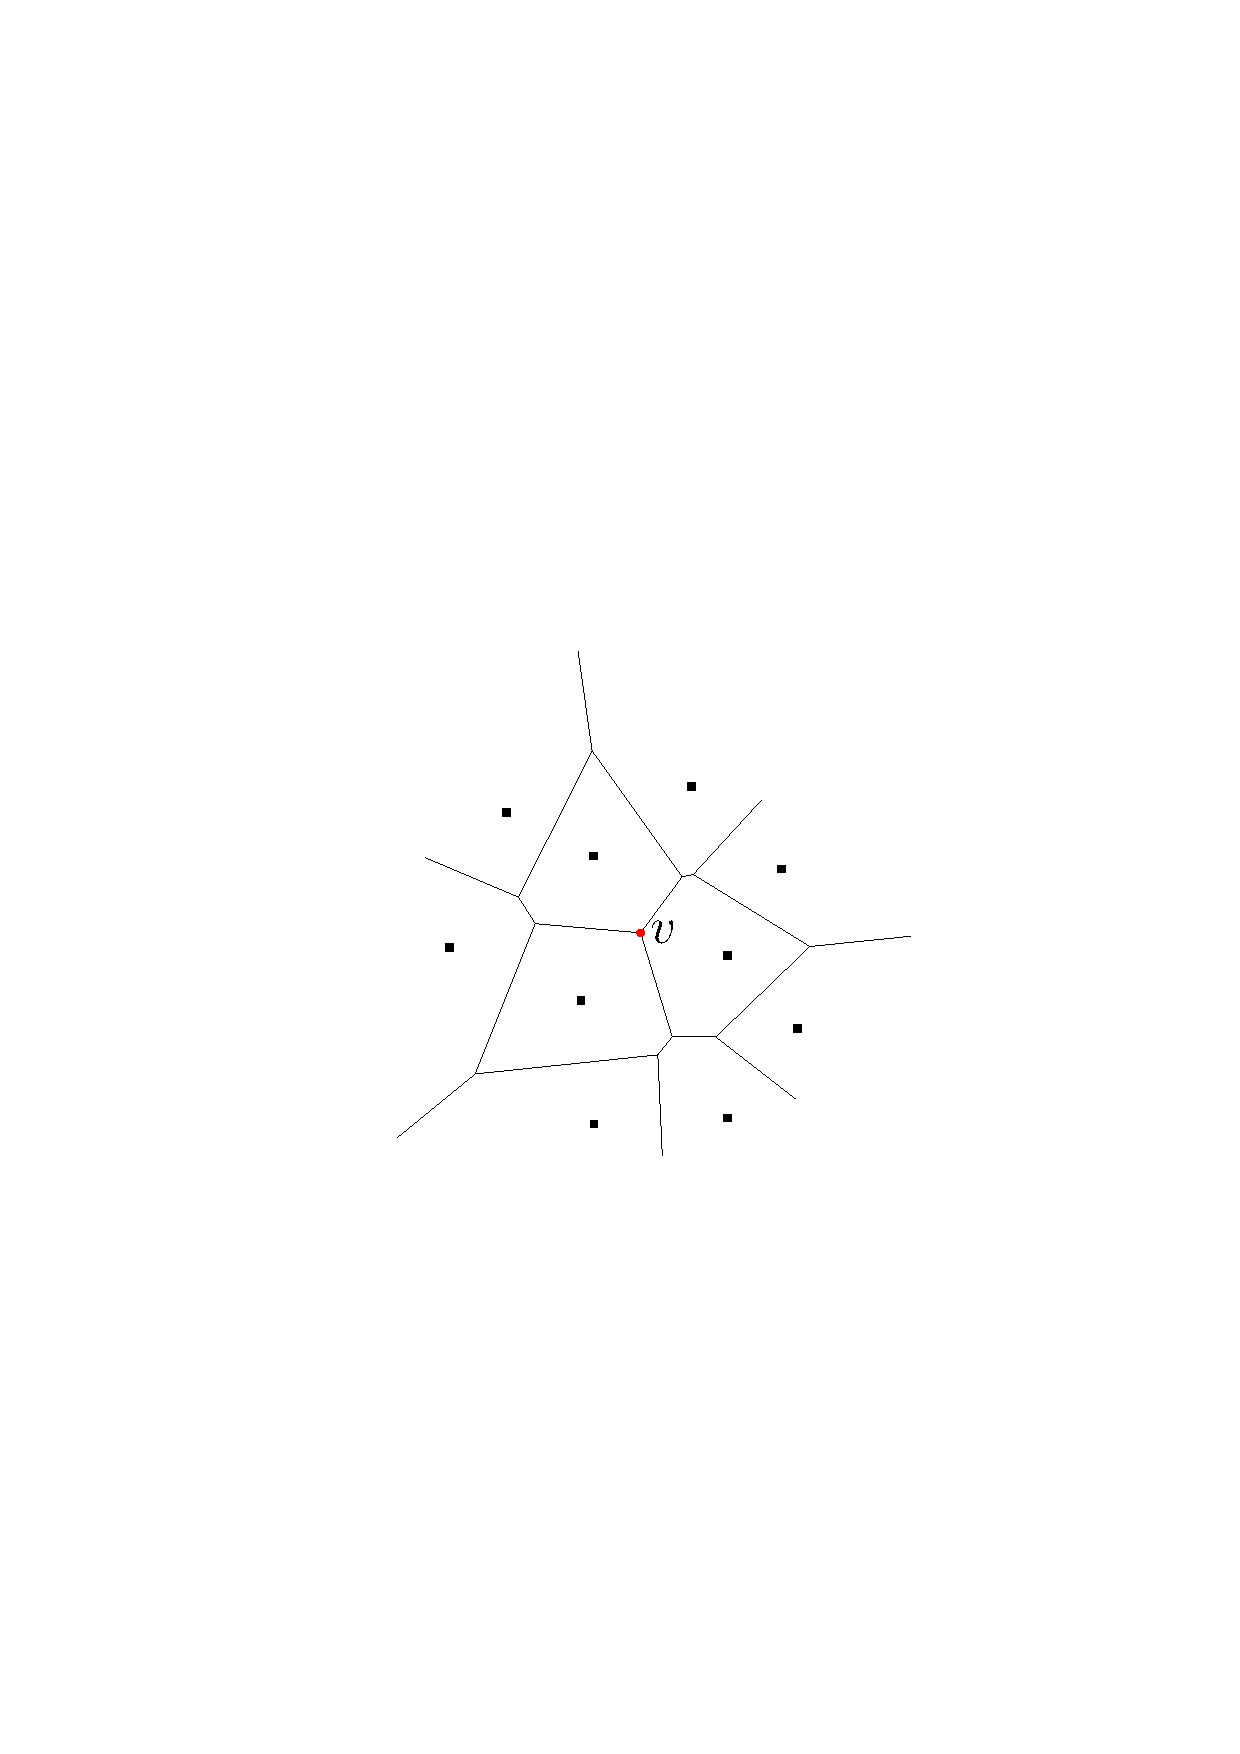
\includegraphics[width=3.7cm]{figs/voronoiDiagram}
	\end{subfigure} \quad
	\begin{subfigure}[t]{0.32\textwidth} \centering
		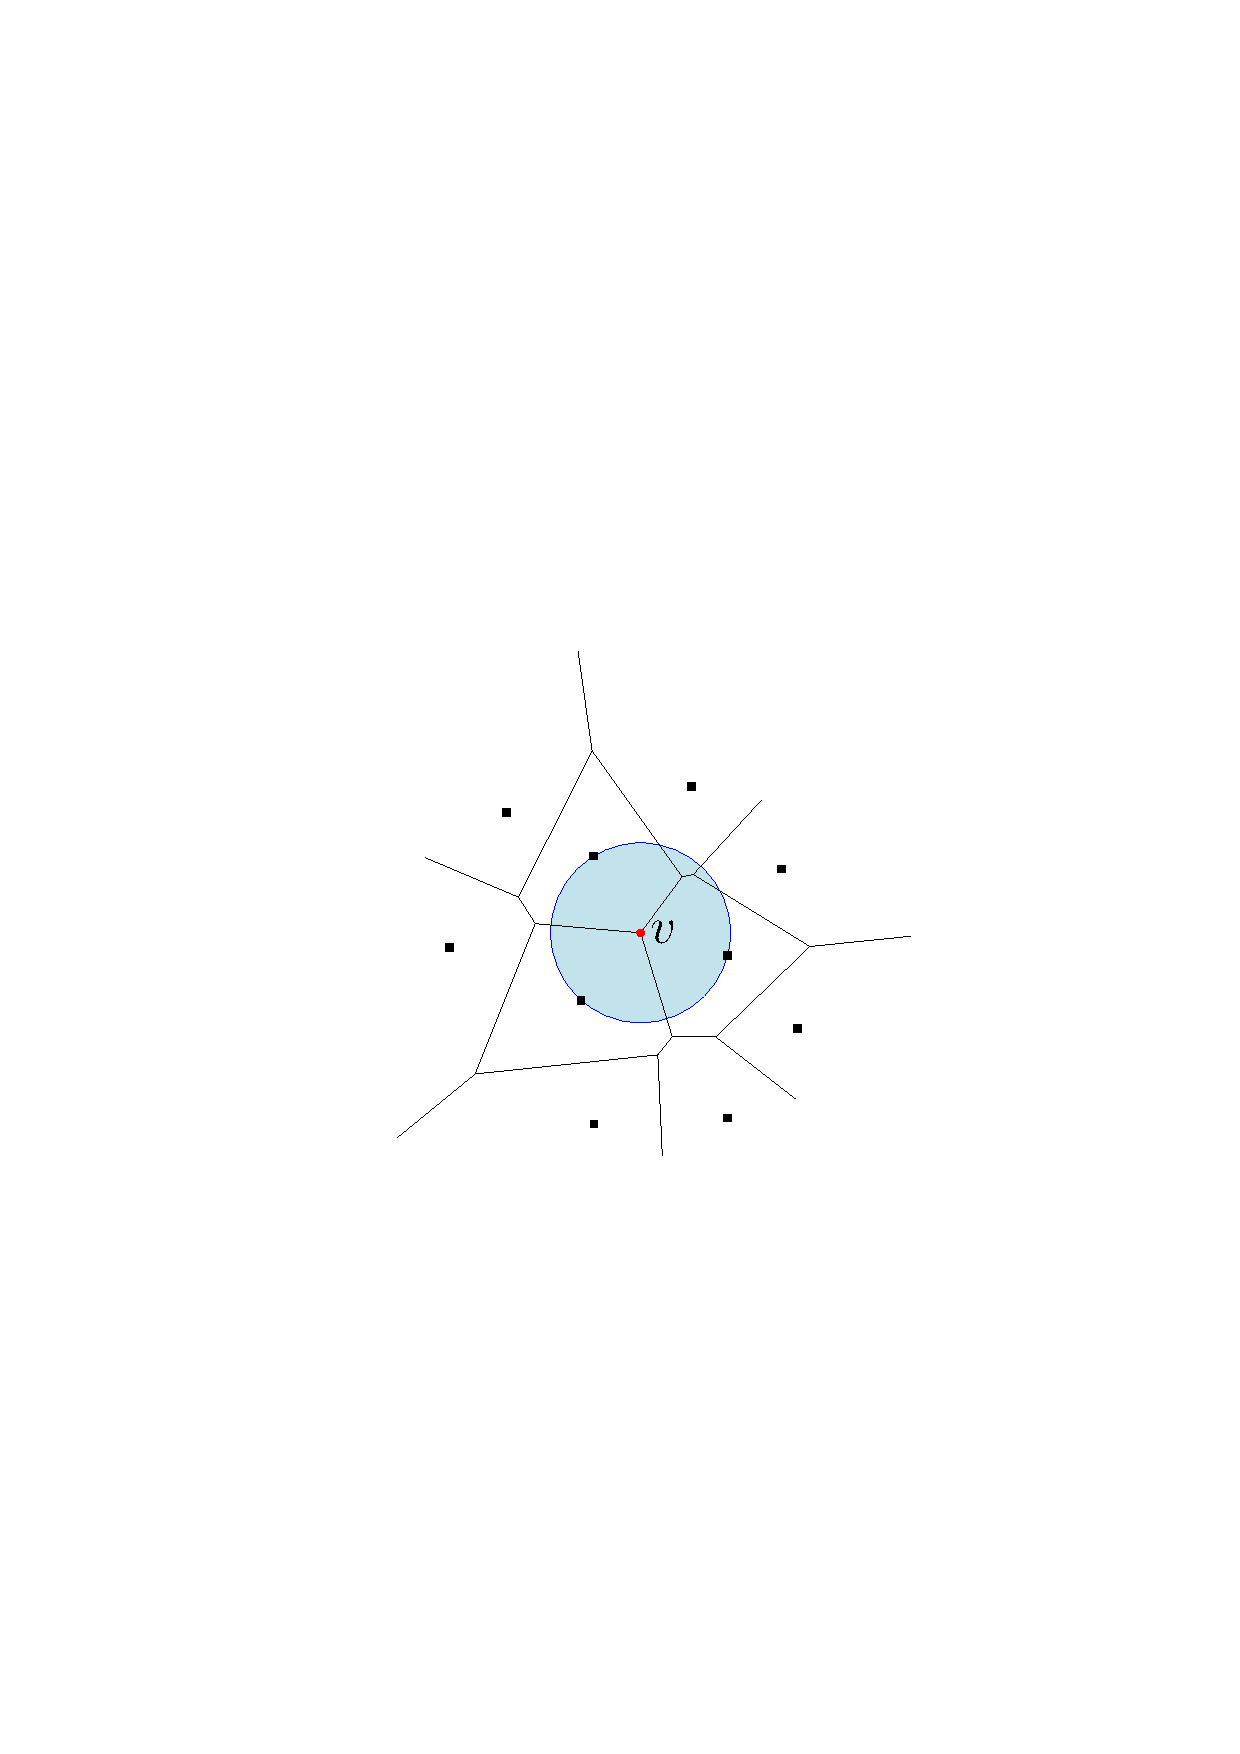
\includegraphics[width=3.7cm]{figs/voronoiCircle}
	\end{subfigure} \quad
\end{figure}

\end{frame}

\begin{frame} \frametitle{Algorithms for Voronoi Diagram}
\begin{enumerate}
	\item Calculate whole Voronoi diagram — $O(n \log n)$: sweep line, divide-and-conquer. \bigskip
	\item (And no better: sorting reduces to Voronoi.) \bigskip
	\item Update the diagram when a new site came — $O(n)$ — {\it literally any} possible way. \bigskip
	\item (And no better: {\it should draw en example here.} There can be that many changes.) \bigskip
	\item But what if we consider {\it the graph} of a diagram...
\end{enumerate}
\end{frame}

\begin{frame} \frametitle{Results today}
\begin{enumerate}
	\item $O(\sqrt{n})$, $\Omega(\sqrt{n})$ edge insertions / removals — even if the diagram is a tree. \bigskip
	
	This is in contrast to $O(n)$ geometric changes and $O(\log n)$ (amortised, existential) combinatorial changes in case of inserting in clockwise order. \bigskip

	\item {\it Algorithm} for insertion of sites in convex position, in arbitrary order — $O(\sqrt{n}\text{ polylog})$.
\end{enumerate}
\end{frame}

\begin{frame} \frametitle{Links and Cuts}
	{\it Link} is the addition of an edge, {\it cut} is the removal of an edge. We count only them. All other operations are thought to have no cost. For example, addition of a vertex. \ps

	How many links / cuts are there in our example?
\end{frame}

\begin{frame} \frametitle{Geometric vs Combinatorial Changes} \label{pg:combvsgeom}
\begin{center}
	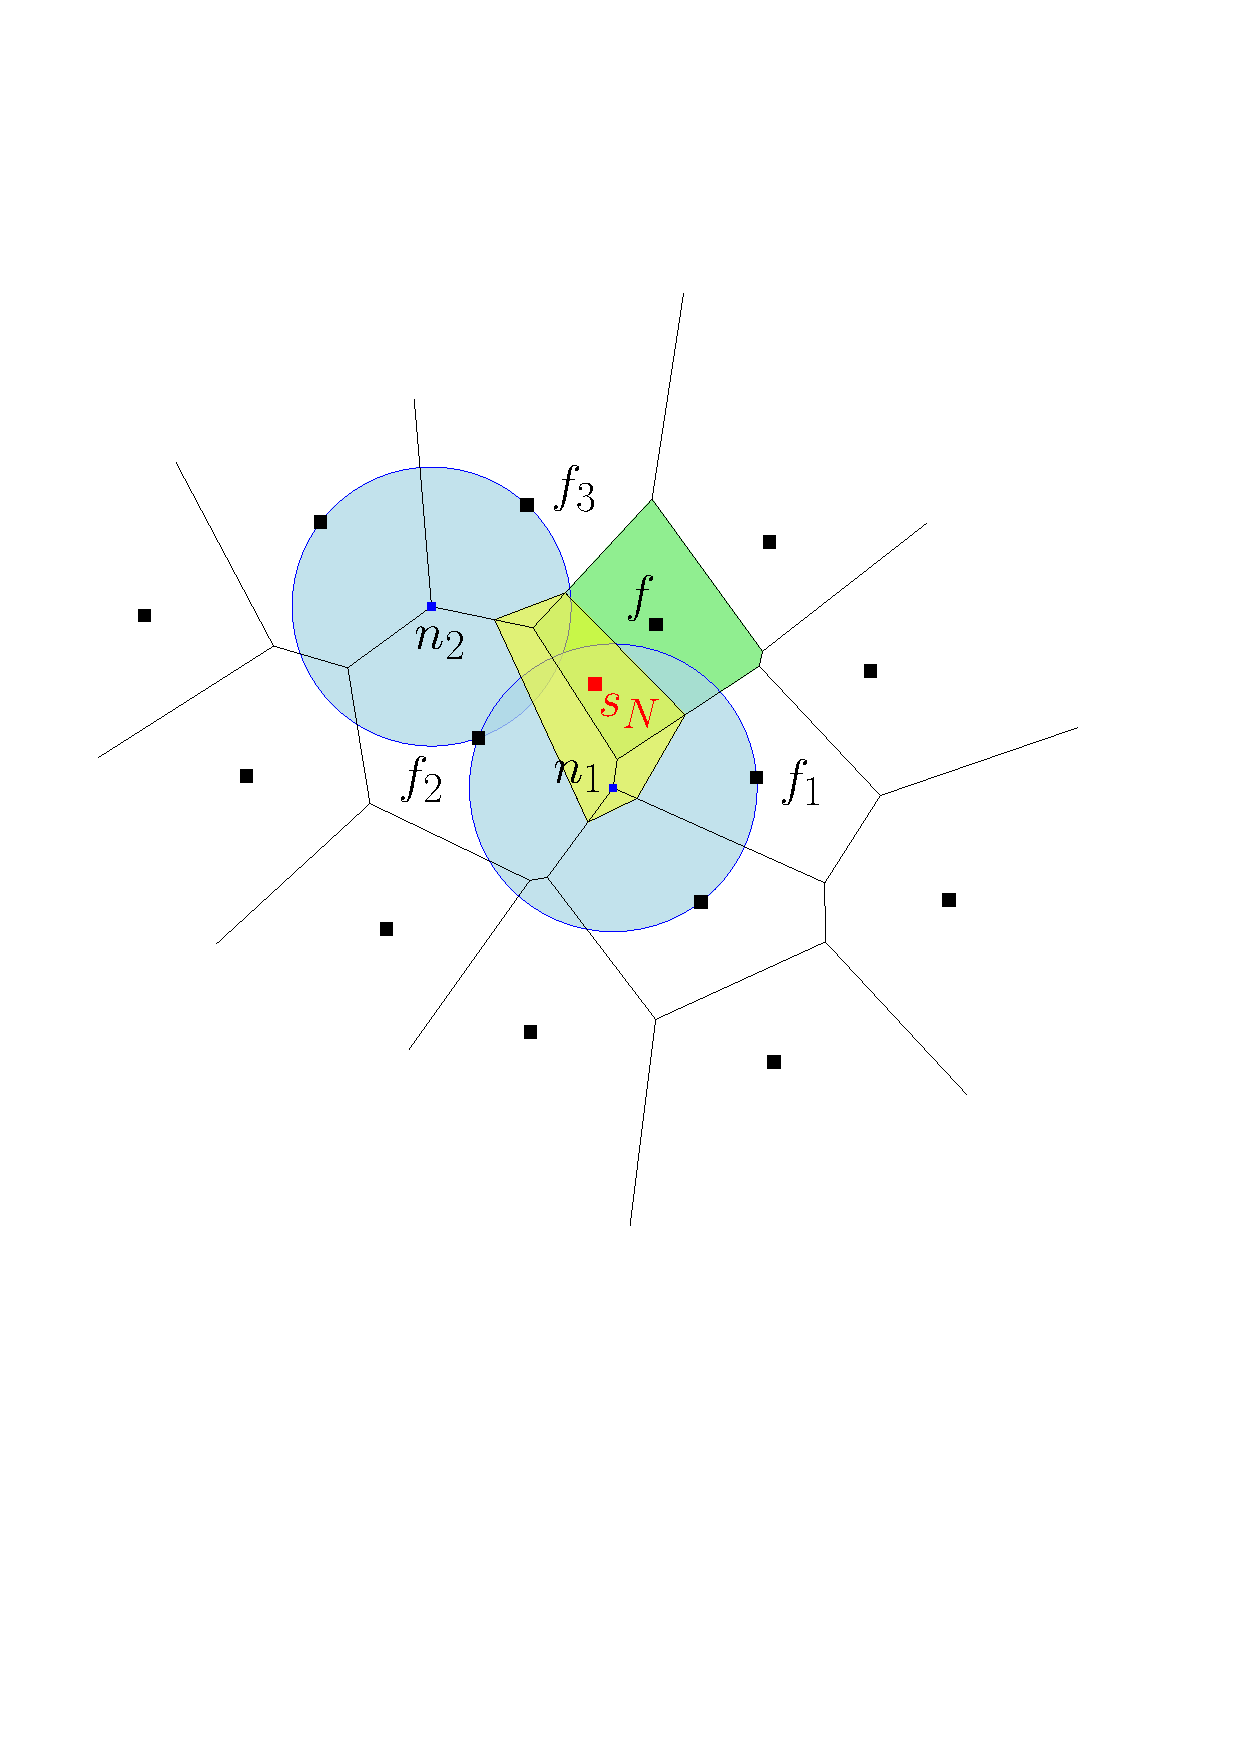
\includegraphics[width=7.4cm]{flarb/identChanges}
\end{center}
\end{frame}

\begin{frame} \frametitle{Chan's structure}
Can be used for:
	\begin{enumerate}
	\item Search of nearest neighbor;
	\item Reporting extreme point in given direction.
	\end{enumerate} \bigskip
Makes use of {\it shallow cuttings.} (Was presented at CG seminar.) Time complexity:
	\begin{enumerate}
	\item Insertion: $O(\log^3 n)$;
	\item Deletion: $O(\log^7 n)$ (improved to $^5$);
	\item Query: $O(\log^2 n)$.
	\end{enumerate}
\end{frame}

\begin{frame} \frametitle{Flarb}
\begin{figure}[h] \centering
	\begin{subfigure}[t]{0.31\textwidth}
	\centering
	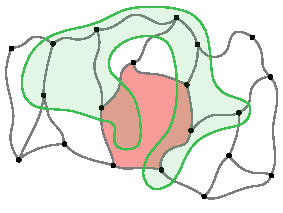
\includegraphics[scale=0.92]{flarb/1notflarb}
	\caption{This curve is not flarbable}
	\end{subfigure}
~
	\begin{subfigure}[t]{0.31\textwidth}
	\centering
	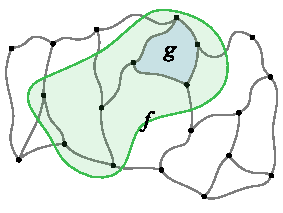
\includegraphics[scale=0.92]{flarb/2flarb}
	\caption{This curve is flarbable}
	\end{subfigure}
~
	\begin{subfigure}[t]{0.31\textwidth}
	\centering
	
\includegraphics[scale=0.92]{flarb/3afterflarb}
	\caption{Result of applying flarb operation}
	\end{subfigure}
\end{figure} \medskip

Fleeq-edges:  those intersecting $\mC$. Note that in a real Voronoi diagram there can be no such cells as $g$.
\end{frame}

\begin{frame} \frametitle{Flarb: Results}
\begin{theorem}
	$\mG(G, \mC)$ has at most two more vertices than $G$ (3-regular graph inside).
\end{theorem} \medskip
\begin{theorem}
	$\mG(G, \mC)$ contains one more face than $G$ (if it comes to Voronoi diagrams).
\end{theorem} \medskip
\begin{theorem}
	For any new point, there exists a curve such that the changes the graph \\
	of V. D. undergoes can be represented by Flarb.
\end{theorem}
\end{frame}

\begin{frame} \frametitle{Preserving operation}
\begin{center}
	Sometimes no links and cuts are needed. \\ \vspace{-0.15cm}
	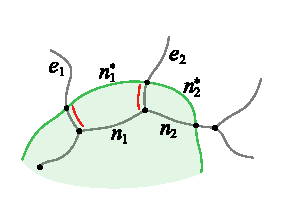
\includegraphics[width=6cm]{flarb/4cost-free}
\end{center} \vspace{-0.6cm}

$\mathcal P(G,\mC)$ — the set of {\it preserved} faces. $\mathcal B(G,\mC)$ — faces wholly inside $\mC$. \\
$\mathcal A(G,\mC)$ — augmented, $\mathcal S(G,\mC)$ — shrinking.
\end{frame}

\begin{frame} \frametitle{Combinatorial Cost of Flarb} \label{pg:flarbcost}
\begin{center}
	{\scshape cost} is how many links / cuts are to be made. \\ \vspace{0.8cm}
	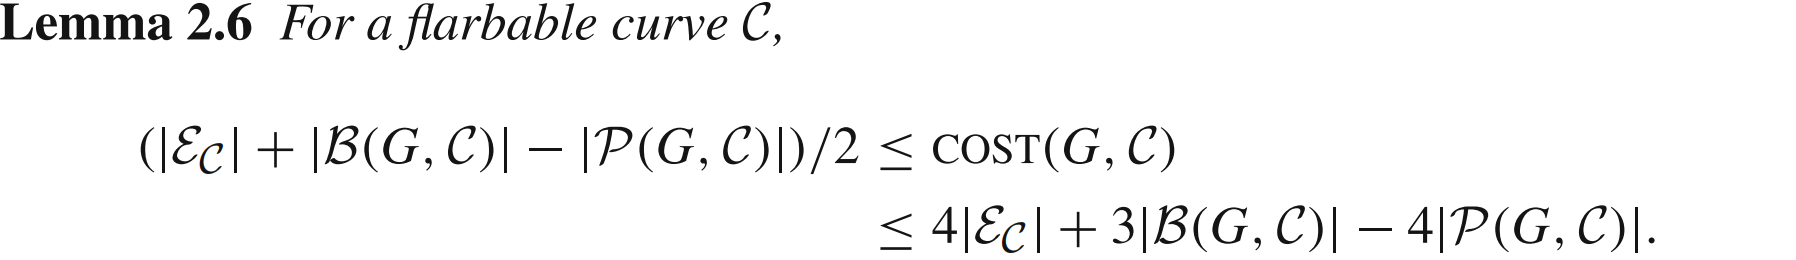
\includegraphics[width=14cm]{figs/2-6.png} \\ \vspace{0.8cm}
	
\includegraphics[width=14cm]{figs/2-8.png}
\end{center}
\end{frame}

\begin{frame} \frametitle{Potential functions}
{\it Amortized complexity analysis} requires a potential function {\it and maybe a couple examples.} \bigskip

\begin{enumerate}
	\item Local:
	$$\mu(f) = \min\left\{ \left\lceil
		\sqrt{\left| V \right|}
	\right\rceil, |f| \right\}.$$ \smallskip
	
	\item Global:
	$$\Phi = \lambda \cdot \sum_f \mu(f).$$
\end{enumerate} \bigskip

Really big faces don't change potential. \\
$\lambda$ will be later set to 24.
\end{frame}

\begin{frame} \frametitle{Flarbable Sub-Curves}
\begin{center}
	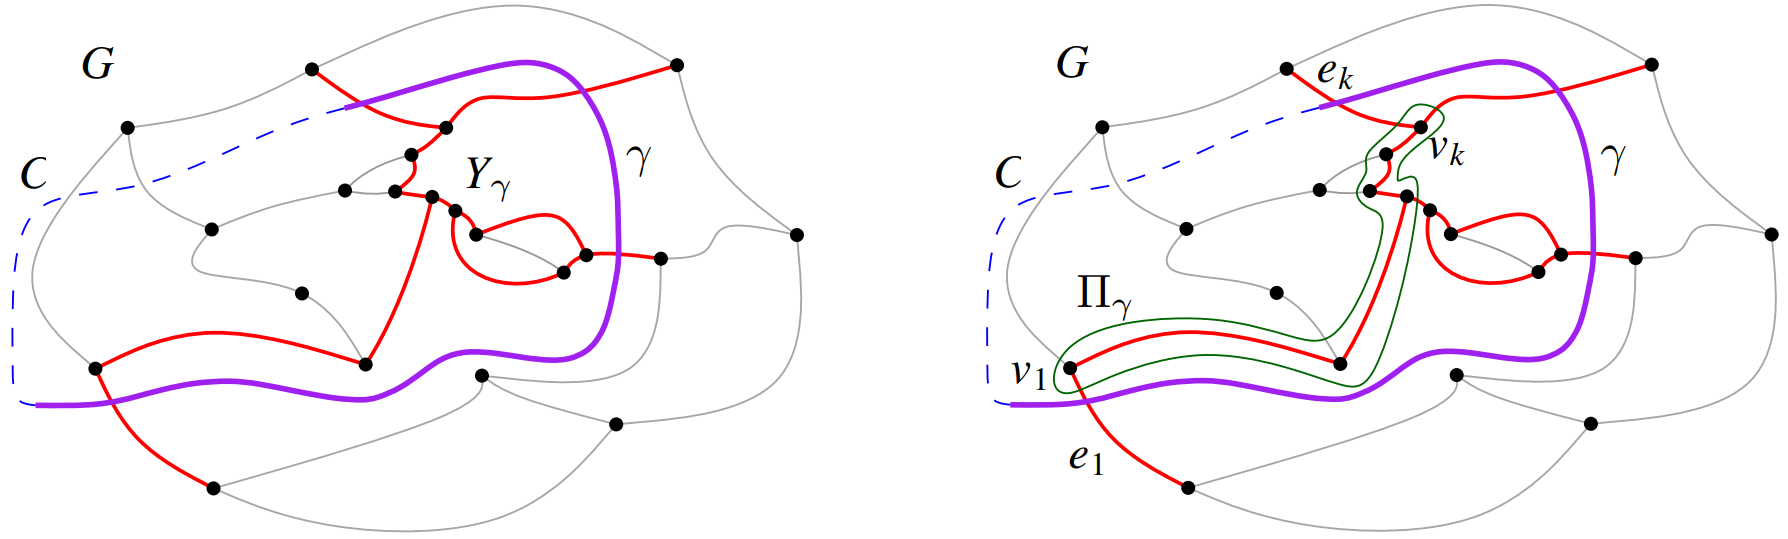
\includegraphics[width=14cm]{figs/subcurve.png} \\ \vspace{0.8cm}
	
\includegraphics[width=14cm]{figs/3-3.png} \\ \vspace{0.4cm}
	
\includegraphics[width=14cm]{figs/3-4.png}
\end{center}
\end{frame}

\begin{frame} \frametitle{Shrinking Faces}
	It turns out that the variation in size of the $\mC$-faces after a flarb \\
	depends only on the number of shrinking faces. \\ \vspace{0.6cm}
\begin{center}
	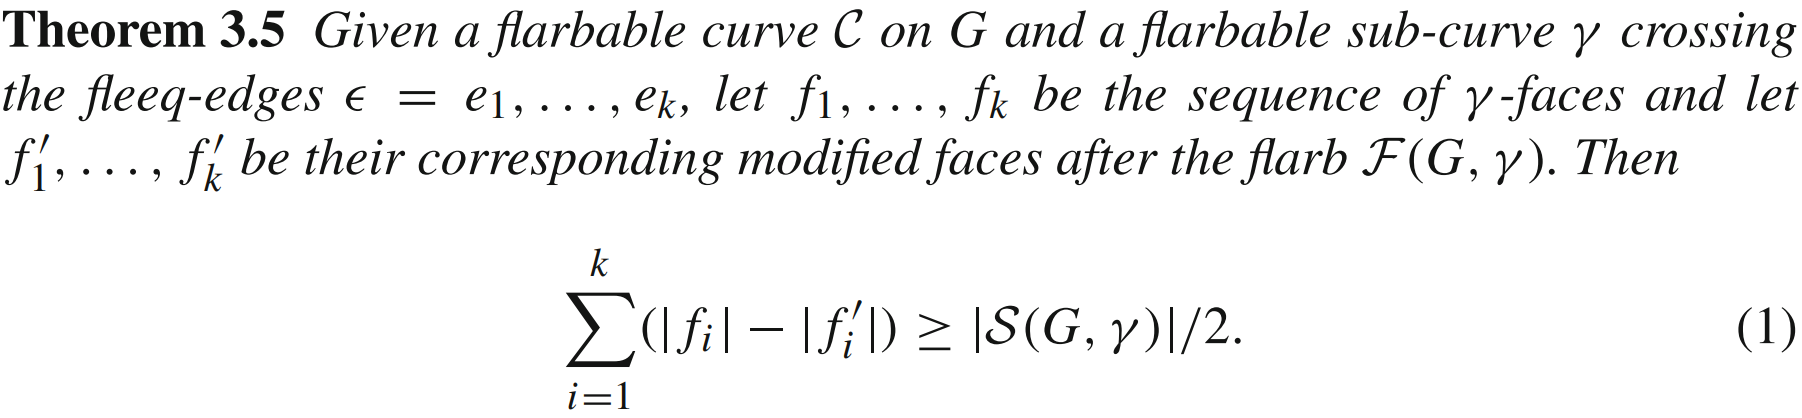
\includegraphics[width=14cm]{figs/3-5.png}
\end{center}
\end{frame}

\begin{frame} \frametitle{Flarbable Sequences} \label{pg:upperbound}
\begin{center}
	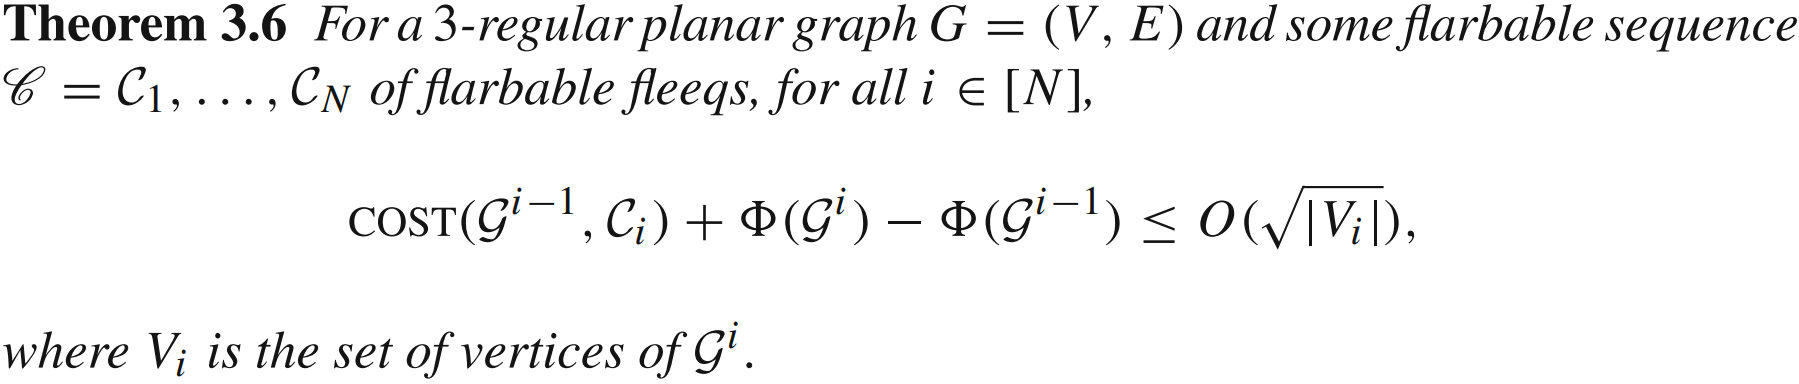
\includegraphics[width=14cm]{figs/3-6.png} \\ \vspace{0.5cm}
	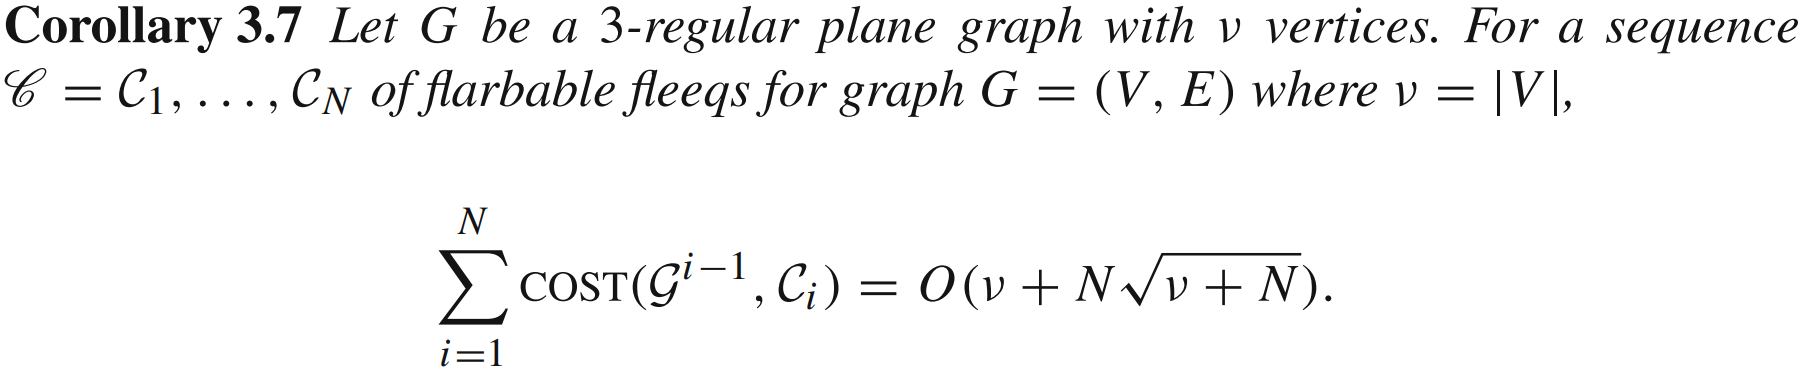
\includegraphics[width=14cm]{figs/3-7.png} \\ \vspace{0.3cm}
	So this is really the amortized bound we needed.
\end{center}
\end{frame}

\begin{frame} \frametitle{Flarbable Sequences}
\begin{center}
	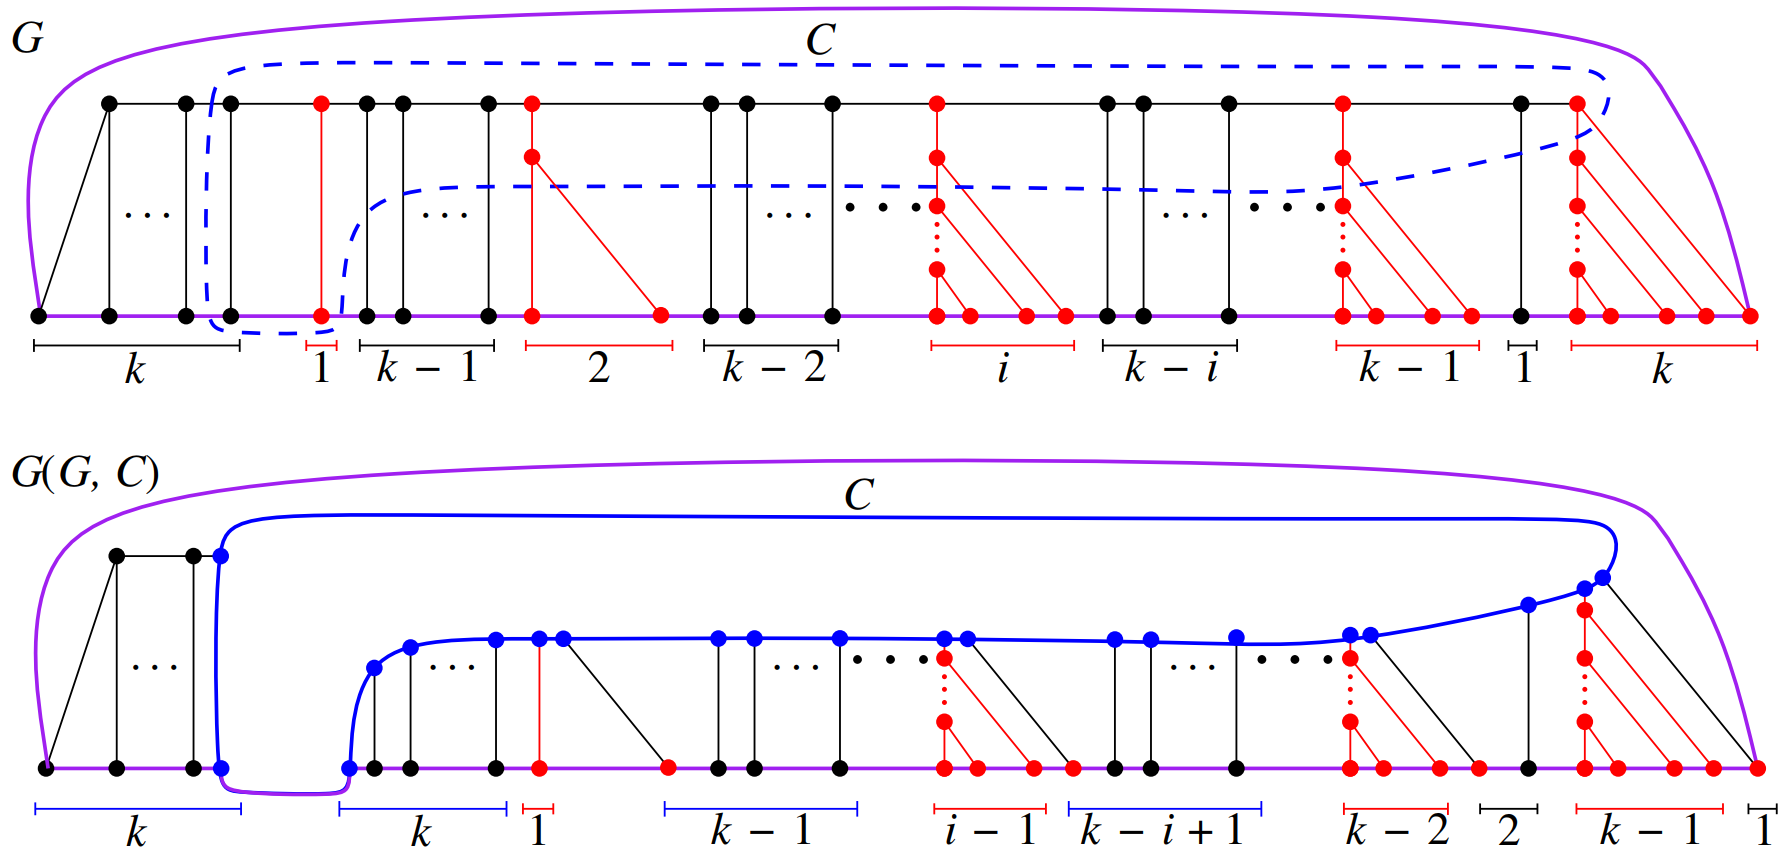
\includegraphics[width=11.75cm]{figs/halin-iso.png} \\ \vspace{0.5cm}
	Flarb produces a graph isomorphic to $G$ and has cost $\Omega \left( \nu \right)$.
\end{center}
\end{frame}

\begin{frame} \frametitle{Grappa Tree}
	A structure designed to store a forest supporting the following operations: \\
	Make-Tree, Link, Cut, Evert, Left-Mark, Right-Mark, Oracle-Search. \\
	Each of them is performed in $O(\log n)$. \\ \bigskip
	Uses heavy-path decomposition. \\ \bigskip
	Voronoi Diagram is stored as a Grappa tree with face-markers \\
	on each edge: cells of which sites are to the right / left from it.
\end{frame}

\begin{frame} \frametitle{Procedure}
\begin{enumerate}
	\item Evert the tree so that the root is at infinity, \medskip
	\item Identify portion of each heavy path inside $\text{\scshape cell} (q, S_{\text{new}})$, \medskip
	\item Within each path find non-preserved edges, \medskip
	\item Remove all non-preserved edges, \medskip
	\item Link back the resulting components in the right order.
\end{enumerate}
\end{frame}

\begin{frame} \frametitle{Dynamic Circle Reporting Structure} \label{pg:dcr}
	We need to report all the circles from the set containing a given point. \\
	Lift the circles to planes
	$$(x,y)\ \mapsto\ (x,y,x^2+y^2).$$ \vspace{-0.4cm}
	
	Using point-plane duality in $\mathbb R^3$ the circle-reporting can be reduced to \\
	extreme-point query that Chan's structure is originally designed for. \bigskip
	
	The DCR has far-going applications. We store roots of heavy paths $\Psi$ \\
	in this structure.
\end{frame}

\begin{frame} \frametitle{Finding Non-Preserved Edges}
	For each root $r \in \Psi_q$ (returned by the DCR) {\it transition edge} $h_r$ is computed in $O(\log n)$. \\ [0.8cm]
\begin{center}
	
\includegraphics[width=14cm]{figs/5-7.png} \\ [0.7cm]
\end{center}
	We can now proceed to finding {\it all} non-preserved edges.
\end{frame}

\begin{frame} \frametitle{Shadow edges. Bent edges.} \vspace{-2mm}
	$\mathcal V_q (S)$ — all the edges of the diagram that intersect the face $\text{\scshape cell} (q, S_\text{new})$ \\
	of new site. \medskip
	
	{\it Shadow edge} is an edge among these that is not preserved. We can mark \\
	all shadow edges in $O(|\Psi_q| \log n)$. There are also {\it bent edges} that can't \\
	be preserved. They need to be marked. 

\begin{center}
	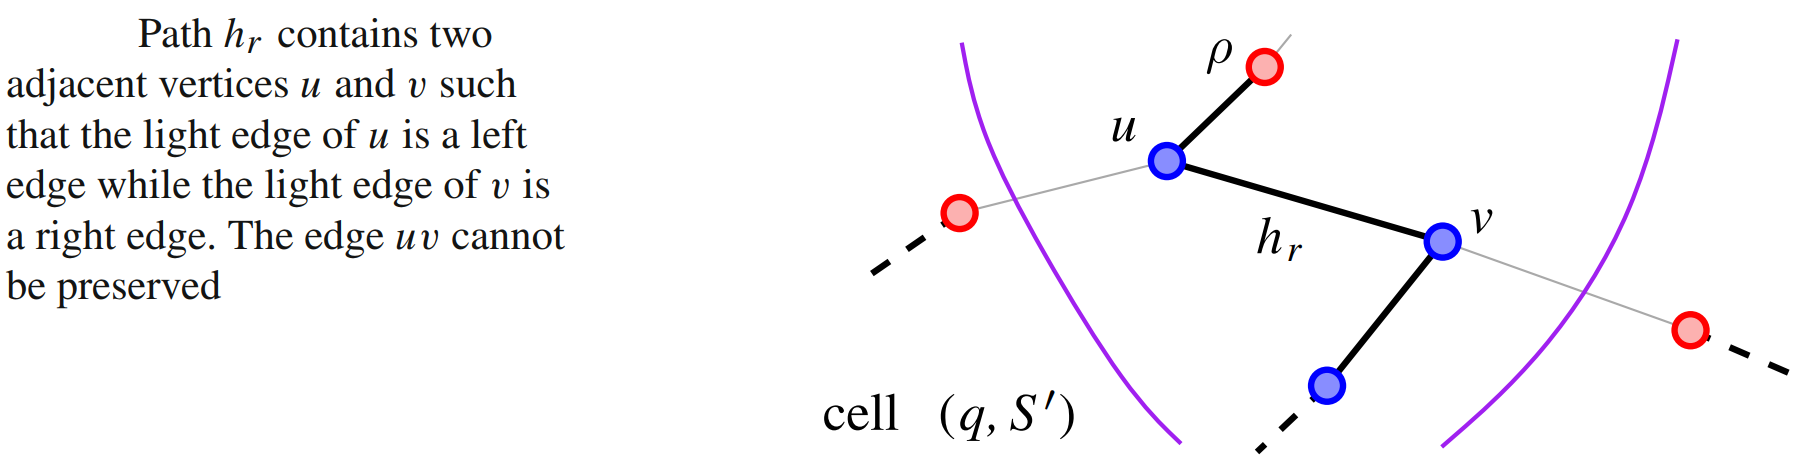
\includegraphics[width=11.5cm]{figs/bent.png} \vspace{-3mm}
\end{center}

	After all, the edge is preserved iff it is not marked as shadow.
\end{frame}

\begin{frame} \frametitle{Compressed Tree} \label{pg:compres}
	$\mathcal F$ — forest obtained after {\it (virtually)} removing all shadow edges. Each component of it is a {\it comb.} Combs can be large, but we want to have a tour on the graph to see how to re-link it. So we compress each comb into a supernode. \medskip

	If $\sigma$ is a number of shadow edges, the compressed tree has $O(\sigma)$ vertices / edges and can be obtained in $O(\sigma \log \sigma)$. \smallskip

\begin{center}
	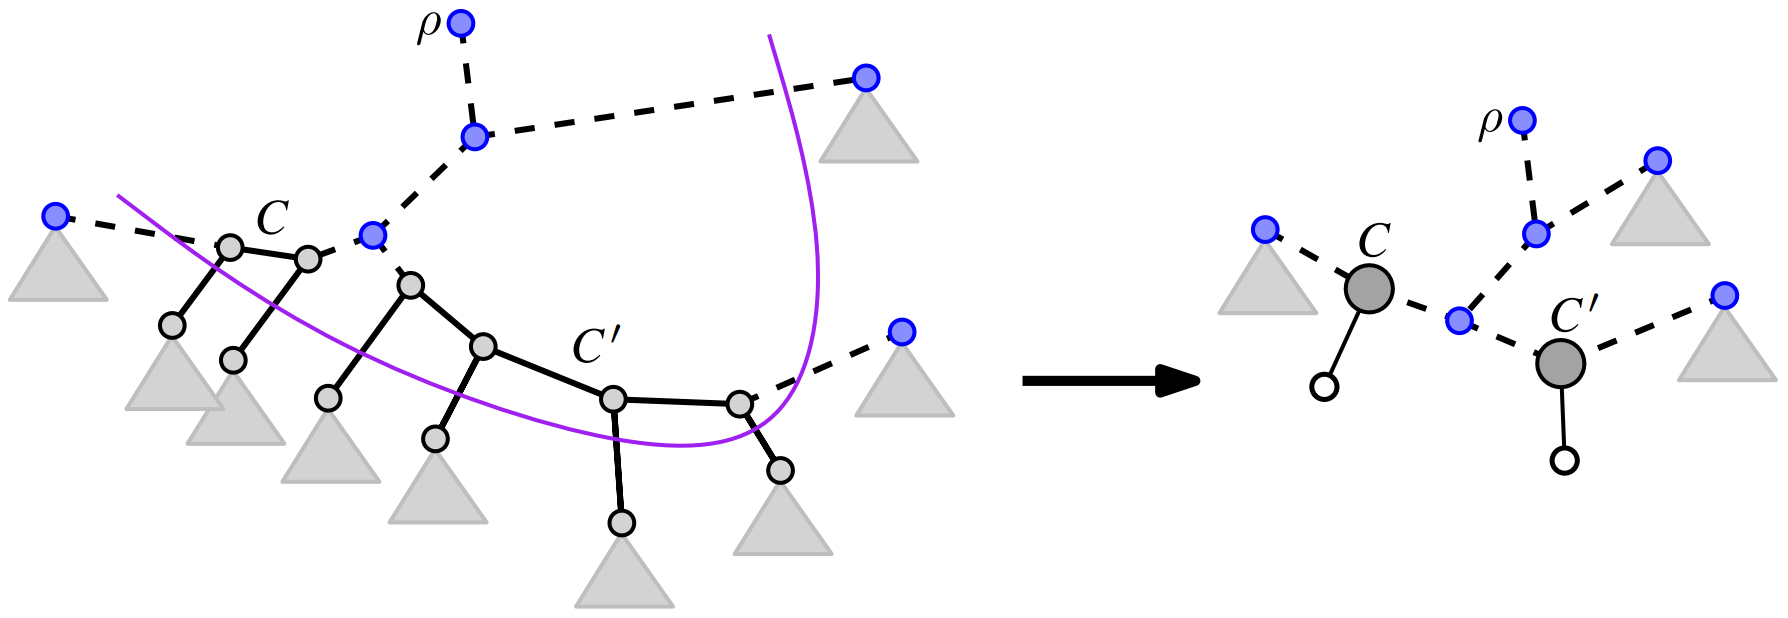
\includegraphics[width=9.8cm]{figs/compres}
\end{center}
\end{frame}

\begin{frame} \frametitle{Decompression}
\begin{center}
	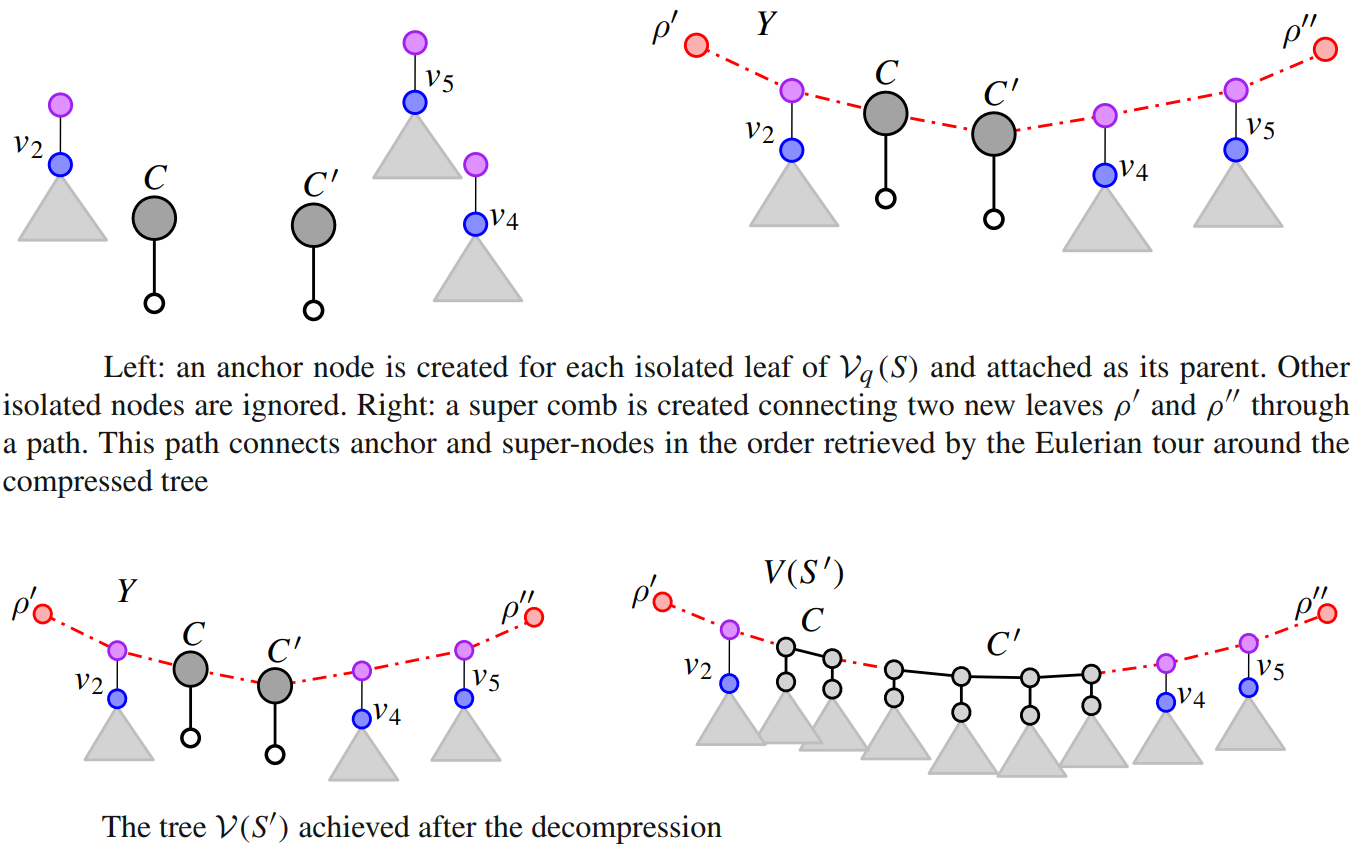
\includegraphics[width=11cm]{figs/decompres}
\end{center}
\end{frame}

\begin{frame} \begin{center} \vspace{0.5cm}
	{\Huge Thank you for your attention!} \\ [1cm]
\end{center}

Main points: \medskip

\begin{enumerate}
	\item Combinatorial vs Geometric changes \hfill Page~\ref{pg:combvsgeom}
	\item Flarb and its combinatorial cost \hfill Page~\ref{pg:flarbcost}
	\item Upper bound $O(\sqrt{n})$ \hfill Page~\ref{pg:upperbound}
	\item Dynamic Circle Reporting \hfill Page~\ref{pg:dcr}
	\item Compression / Decompression \hfill Page~\ref{pg:compres}
\end{enumerate}
\end{frame}

\end{document}